% !TEX root = ../main.tex
% chktex-file 21
% chktex-file 46
\section{Introduction}%
\label{sec:intro}

\pagenumbering{arabic}			% arabic page numbering
\setcounter{page}{1}			% set page counter

With the rise of Big Data applications over the recent years, working with large graph structures also became more important.
Algorithms like PageRank or spectral clustering are commonly used to analyze the web graph or social networks.
In order to run such algorithms on large graphs however, optimizations are required.

For this purpose we will specifically look at graph coarsening.
Coarsening reduces the size of a given graph while preserving its overall structure via some notion of graph similarity that will be defined later.
Graph algorithms can then be run on the smaller coarsened graph.
Afterwards the result for the coarsened graph can be iteratively refined to obtain an approximate result for the original graph.
Figure~\ref{fig:intro:overview} illustrates this approach.
\begin{figure}
	\centering
	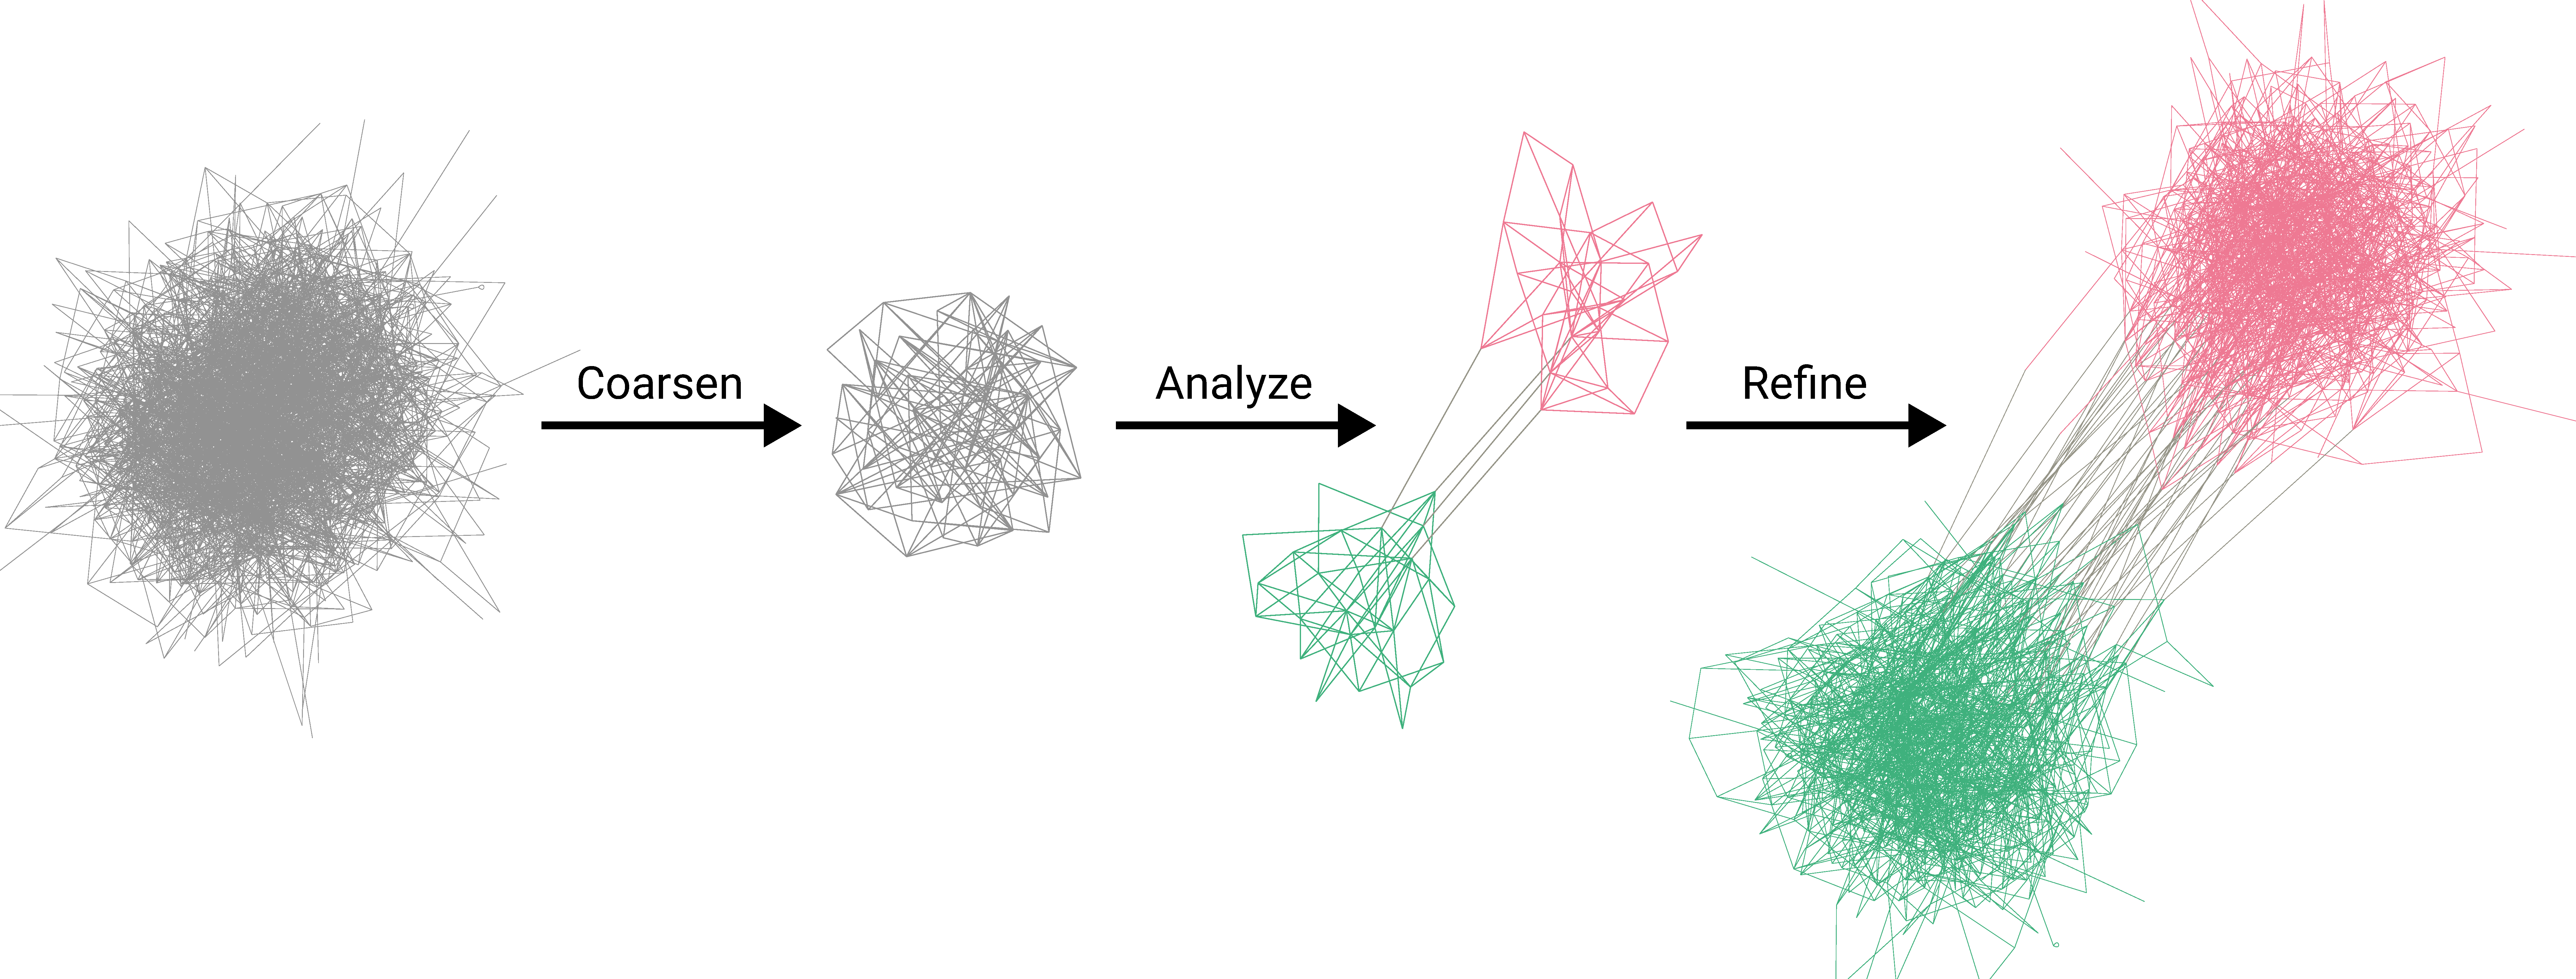
\includegraphics[width=0.8\linewidth]{gfx/intro/overview.pdf}
	\caption{
		Using graph coarsening to speed up graph algorithms, e.g.\@ Min-Cut.
	}\label{fig:intro:overview}
\end{figure}

The goal of this paper is to show how graph coarsening works and how it affects the results of graph algorithms.
This introduction consists of three sections, each of which aims to answer one main question:
\begin{enumerate}
	\item \textit{How can the structural properties of a graph be formally described?}
		To describe graph coarsening and its effects, the similarity between a graph $G$ and its coarsened version $G_c$ has to be quantified.
		We begin with an introduction to spectral graph theory.
		It allows us to describe the structure of graphs and provides the notion of the \textit{graph spectrum}, a way to describe the overall structure of graphs.
	\item \textit{How does graph coarsening work?}
		Based on the notion of the graph spectrum, we will look at a randomized coarsening algorithm and analyze its effects on the structure of the coarsened graph.
	\item \textit{How does coarsening affect the result of graph algorithms?}
		Finally we will put bounds on how much the described coarsening algorithm is expected to increase the error of spectral clustering.
\end{enumerate}
